\section{线性求解}\label{sec:lin_solver}

通过算法~\ref{alg:schur_update}更新舒尔补方程后,可以通过求解舒尔补方程快速得到相机状态的增量$\bm{\delta}^c$,再进一步通过回代求解三维点状态的增量$\bm{\delta}^l$。为了提升这部分求解数值稳定性,本文提出了使用混合式LM-DL方法(Hybrid Levenberg-Marquardt-Dog-Leg,简称HLMDL)求解舒尔补方程。在回代求解部分,受iSAM2\citep{kaess2012isam2}算法的启发,本文提出了使用部分贝叶斯推断树(Partial Bayes Tree,简称PBT)的方法编码三维点状态和相机状态之间的推断关系,以达到增量式回代的目的,进一步提高效率。

\subsection{传统DL算法}

LM法的阻尼因子会影响正规矩阵的对角线元素,经过舒尔补操作之后,阻尼因子的影响被不可逆地累积到了舒尔补矩阵中,使得每次调整阻尼因子的时候必须要重新完整计算舒尔补。这会导致舒尔补无法进行增量更新,因此ICE-BA\citep{liu2018ice}和SLAM++中均使用DL法进行非线性求解。第~\ref{ch:intro}~章已经介绍了DL算法的基本策略,算法~\ref{alg:dogleg}给出了传统DL算法的详细步骤。

\begin{algorithm}[htb!]
\caption{Dog-Leg法}
\begin{algorithmic}
    \Require 初始信赖域半径$\Delta_0$,初值$\bm{x}_0$
    \Ensure 优化结果$\bm{x}$

    \State $\Delta \coloneqq \Delta_0, \bm{x} \coloneqq \bm{x}_0$
    \For{$k = 0 \rightarrow k_{max}$}
        \State $k \coloneqq k+1$
        \State 使用式\eqref{eq:lls}计算线性化子问题
        \State 使用式\eqref{eq:gn}计算高斯-牛顿迭代步$\bm{\delta}_{gn}$
        \State 使用式\eqref{eq:sd}计算最速下降迭代步$\bm{\delta}_{sd}$
        \State 使用式\eqref{eq:dl}计算DL法步长$\bm{\delta}_{dl}$

        \If{\{步长$\bm{\delta}_{dl}$收敛\}}
            \State 结束优化
        \EndIf

        \State 计算迭代步质量$\varrho$:
        \[
            \varrho = \frac {F(\bm{x})-F(\bm{x}+\bm{\delta}_{dl})}
                            {L(\bm{0})-L(\bm{\delta}_{dl})}
        \]

        \If{\{$\varrho > 0.0$\}}
            \State $\bm{x} \coloneqq \bm{x} + \bm{\delta}_{dl}$
        \EndIf

        \If{\{$\varrho > \epsilon_0$\}}
            \State $\Delta \coloneqq \text{fmax}\{\Delta,3\left\|\bm{\delta}_{dl}\right\|\}$
        \ElsIf{\{$\varrho < \epsilon_1$\}}
            \State $\Delta \coloneqq \Delta/2$
        \EndIf

        \If{\{信赖域$\Delta$收敛\}}
            \State 结束优化
        \EndIf
    \EndFor
\end{algorithmic}
\label{alg:dogleg}
\end{algorithm}


\subsection{HLMDL方法求解舒尔补方程}

然而如第~\ref{ch:intro}~章中提到的,在实际求解线性问题时,往往会遇到矩阵秩亏或不正定的情况,而且这种情况在舒尔补矩阵中更为严重,这就造成了直接求解时数值不稳定的问题。为了避免这个问题,本文提出了改进,使用HLMDL的方法,在舒尔补矩阵的对角线上加上阻尼因子:
\begin{equation}
    \mathrm{S}' \doteq \mathrm{S}+\mu\mathbf{diag}(\mathrm{S})
\end{equation}
来改善舒尔补矩阵的秩亏现象。然后通过求解新的舒尔补方程得到相机状态增量$\bm{\delta}^c$:
\begin{equation}
    \bm{\delta}^c = \mathrm{S}' \:\setminus\: \bm{b}
    \label{eq:hlmdl}
\end{equation}
最后从$\mathrm{S}'$中减去阻尼因子的影响,恢复为原先的舒尔补矩阵:
\begin{equation}
    \mathrm{S} = \mathrm{S}'-\mu\mathbf{diag}(\mathrm{S})
\end{equation}
由于阻尼因子直接施加在构建好的舒尔补矩阵上而非原始的正规矩阵$\mathrm{H}$,其影响是可逆的,经过简单的操作即可恢复,在下一轮迭代中仍可以使用增量式方法更新舒尔补方程。通过HLMDL方法求得的$\bm{\delta}^c$是原始舒尔补方程的一个近似解,但是由于使用了迭代的方式求解,单次迭代的近似解对最终的结果影响很小。这里的阻尼因子的调整与DL的信赖信赖的调整是独立的,本文使用了\citen{tingleff2004methods}中的方法进行阻尼调节,逐步缩小阻尼因子,使得最后的解收敛于准确的解。

方程\eqref{eq:hlmdl}的求解可以使用任何常用的矩阵分解法,如QR分解、Cholesky分解等。也可以采用迭代式的线性求解方法,比如预处理共轭梯度法(preconditioned conjugate gradient,简称PCG)。本文提出的框架提供了自定义线性求解方法的接口,用户可以自己实现符合实际数值稳定性需求和求解效率要求的线性求解方法,也可以使用内置的Cholesky分解求解器和I-PCG求解器。

由于HLMDL方法在舒尔补方程上施加了阻尼因子,本文没有使用增量式Cholesky分解\citep{polok2013incremental}来求解式\eqref{eq:hlmdl},而是提供了常规的Cholesky分解法和ICE-BA中提出的I-PCG方法,并配合Jacobi预处理方法\citep{jeong2012pushing}来提升线性求解的效率。算法~\ref{alg:hlmdl}描述了HLMDL算法的一次迭代过程。

\begin{algorithm}[htb!]
\caption{一轮HLMDL算法迭代}
\begin{algorithmic}
    \Require 舒尔补方程$\mathrm{S}$,$\bm{b}$,阻尼因子$\mu_i$
    \Ensure 本轮迭代结果$\bm{\delta}^c$,下一轮阻尼因子$\mu_{i+1}$

    \State 对舒尔补矩阵施加阻尼因子
    \[
        \mathrm{S}' \doteq \mathrm{S}+\mu\mathbf{diag}(\mathrm{S})
    \]

    \State 使用Cholesky分解或I-PCG方法求解新的舒尔补方程
    \[
        \bm{\delta}^c = \mathrm{S}' \:\setminus\: \bm{b}
    \]

    \State 恢复舒尔补矩阵
    \[
        \mathrm{S} = \mathrm{S}'-\mu\mathbf{diag}(\mathrm{S})
    \]

    \State 使用\citen{tingleff2004methods}中的方法调节阻尼因子$\mu_i$,得到$\mu_{i+1}$
\end{algorithmic}
\label{alg:hlmdl}
\end{algorithm}


\subsection{使用PBT方法增量回代}

ICE-BA中使用了直接回代的方法求解三维点状态的增量,即求解完相机状态增量$\bm{\delta}^c$后,进一步使用式\eqref{eq:back_sub}直接批量回代求解三维点状态的增量$\bm{\delta}^l$。最后得到的总的状态增量$\bm{\delta}$,通过阈值判断其每个分量$\bm{\delta}_i$是否发生了足够大的更新并将发生较大更新的分量更新到状态中:
\begin{equation}
    \bm{x}_i \leftarrow \bm{x}_i + \bm{\delta}_i, \quad
    \forall \left\|\bm{\delta}_i\right\|_{\infty} \geq \varepsilon
\end{equation}

这一步求解并不是增量进行的,除了计算速度受到一定的影响,还存在变量更新不一致的问题。一种典型的情况是:某个相机状态$i$的增量$\bm{\delta}^c_i$较小,而与之相关的某个三维点状态$j$的增量$\bm{\delta}^l_{j}$发生了较大的更新,此时对应的因子$f(\bm{x}^c_i,\bm{x}^l_j)$被标记为脏因子,需要重新线性化$f(\bm{x}^c_i+\bm{\delta}^c_i,\bm{x}^l_j+\bm{\delta}^l_j)$,但由于$\bm{\delta}^c_i$较小而被忽略,实际计算的是$f(\bm{x}^c_i,\bm{x}^l_j+\bm{\delta}^l_j)$。这就造成变量更新的不一致,在实际运行过程中,会导致增量求解过程中能量收敛的变慢,影响求解效率。

针对这一情况,本文基于iSAM2算法的贝叶斯推断树方法提出了PBT方法,编码了三维点状态和相机状态之间的推断关系。iSAM2算法认为通过高斯消元法进行Cholesky分解或QR分解过程对应了将因子图转化为贝叶斯推断树的过程,贝叶斯推断树编码了所有变量之间的推断关系。在求解完根节点对应的变量之后,需要从根节点开始递归地回代求解叶节点。如果某个节点的变量的更新较小,则停止回代,其所有后代节点均不再继续回代求解(即使其中仍有可能有潜在的更新较大的节点)。这一操作使得整个回代求解过程与变量推断关系严格一致。

构建舒尔补的过程实际也是使用高斯消元将一部分变量(三维点状态)进行消去的过程,同样这个过程也可以生成贝叶斯推断树。以因子图~\ref{fig:factor_graph}为例,其舒尔补过程可以生成如图~\ref{fig:bayes_forest}所示的贝叶斯推断树。由于舒尔补只消去了三维点状态,而相机状态部分则保留原始状态,因此构建的贝叶斯推断树为部分贝叶斯推断树$\mathcal{T}_p$(Partial Bayes Tree,简称PBT),高度固定为$2$,所有相机变量共同构成了根节点$Rt(\mathcal{X})$,每一个叶节点$L(l_i|\mathcal{S}_i)$代表一个三维点状态$l_i$及其前置条件状态集合$\mathcal{S}_i$。

\begin{figure}[htb!]
    \centering
    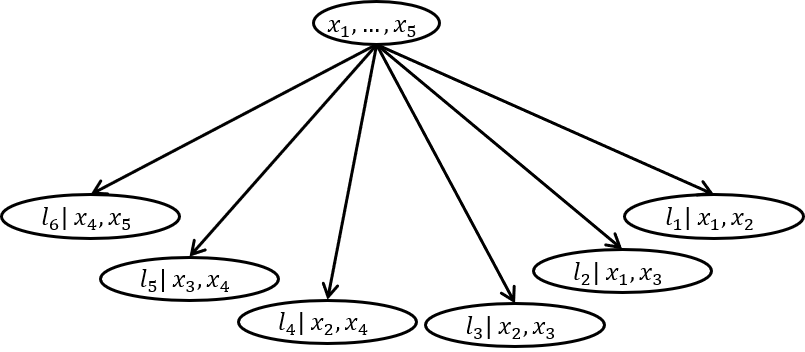
\includegraphics[scale=.9]{Pictures/bayes_forest.png}
    \caption{舒尔补构建的贝叶斯推断树}
    \label{fig:bayes_forest}
\end{figure}

利用PBT,可以方便地推断出任意一个三维点状态的前置条件变量。如果某个相机状态变量没有更新或更新较小,则以其为前置条件的三维点状态也不会更新(即使该三维点可能也发生了较大更新)。这就保证了三维点状态的更新和相机状态的更新的一致性。

\begin{algorithm}
\caption{PBT回代算法}
\begin{algorithmic}
    \Require PBT树$\mathcal{T}_p$,相机状态增量$\bm{\delta}^c$
    \Ensure 三维点状态增量$\bm{\delta}^l$
    \State{$\bm{\delta}^l \coloneqq \bm{0}$}
    \ForAll{叶子节点$L(l_i|\mathcal{S}_i)\in\mathcal{T}_p$}
        \State{记$\mathcal{S}_i$对应的相机状态增量为$\bm{\delta}^c_{S_i}$}
        \If{\{$\left\|\bm{\delta}^c_{S_i}\right\|_{\infty} < \varepsilon$\}}
            \State $\bm{\delta}^l_i \coloneqq \bm{0}$
        \Else
            \State $\bm{\delta}^l_i \coloneqq \bm{l}_i$
            \ForAll{\{$\bm{\delta}^c_j\in\mathcal{S}_i$\}}
                \State
                {
                    $\bm{\delta}^l_i \coloneqq
                     \bm{\delta}^l_i - \mathrm{W}^\top_{ji}\bm{\delta}^c_j$
                }
            \EndFor
            \State
            {
                $\bm{\delta}^l_i \coloneqq
                 \mathrm{P}_{ii}^{-1} \bm{\delta}^l_i$
            }
        \EndIf
    \EndFor
\end{algorithmic}
\label{alg:pbt}
\end{algorithm}



算法~\ref{alg:pbt}介绍了PBT回代的基本步骤。通过PBT回代求解得到$\bm{\delta}^l$后,进一步地,如果还需要进行下一轮迭代,则将综合更新量$\bm{\delta}$传递给算法~\ref{alg:mark_dirty},计算新一轮的迭代。整个增量舒尔补和线性求解的过程均可以基于块状稀疏矩阵实现。相比与稠密矩阵或一般的稀疏矩阵算法,块状稀疏矩阵的计算过程对cache更友好,也更适合使用CPU浮点指令集加速。得益于块状稀疏矩阵的高效,整个增量式集束调整的效率相比批量式集束调整可以有非常大的提升。
